\documentclass{article}

\usepackage{authblk}
\usepackage{graphicx}
\usepackage{subfig}


\title{Supplemental Material: A multi-modal neural network for learning cis and trans regulation of stress response in S. cerevisiae}

\author[1,2,3]{Boxiang Liu}
\author[4]{Nadine Hussami}
\author[3,5]{Avanti Shrikumar}
\author[3]{Tyler Shimko}
\author[6]{Salil Bhate}
\author[6]{Scott Longwell}
\author[2,3]{Stephen Montgomery}
\author[3,6]{Anshul Kundaje}
\affil[ ]{$^1$Departments of Biology, $^2$Pathology, $^3$Genetics, $^4$Statistics, $^5$Computer Science, and $^6$Bioengineering, Stanford University}
\affil[ ]{\textit{\{bliu2,nadinehu,avanti,tshimko,bhate,longwell,smontgom,akundaje\}@stanford.edu}}

\begin{document}

\maketitle

\tableofcontents

\listoffigures

\section{Yeast Microarray Data}
\label{sec: Yeast Microarray Data}
In this study we used transcriptome microarray measuring cDNA abundance by Gasch et al\cite{Gasch:2000wl}. In total, there are 6110 genes across 173 experimental conditions. The dataset were given as as $log_2$ fold change w.r.t an unstimulated reference expression. We decided not to performance further normalization to preserved the interpretation of true zero, i.e. no change w.r.t the reference. We selected 472 signaling molecules and transcription factors as input the regulatory module (see Section \ref{sec: Neural Network Architecture}). We used 1kbp promoter sequence directly upstream of the TSS as input to the sequence module. The data can be visualized in graphical form as follows. Each column represent a experimental condition, and each row is a gene. 

\begin{figure}
\centering
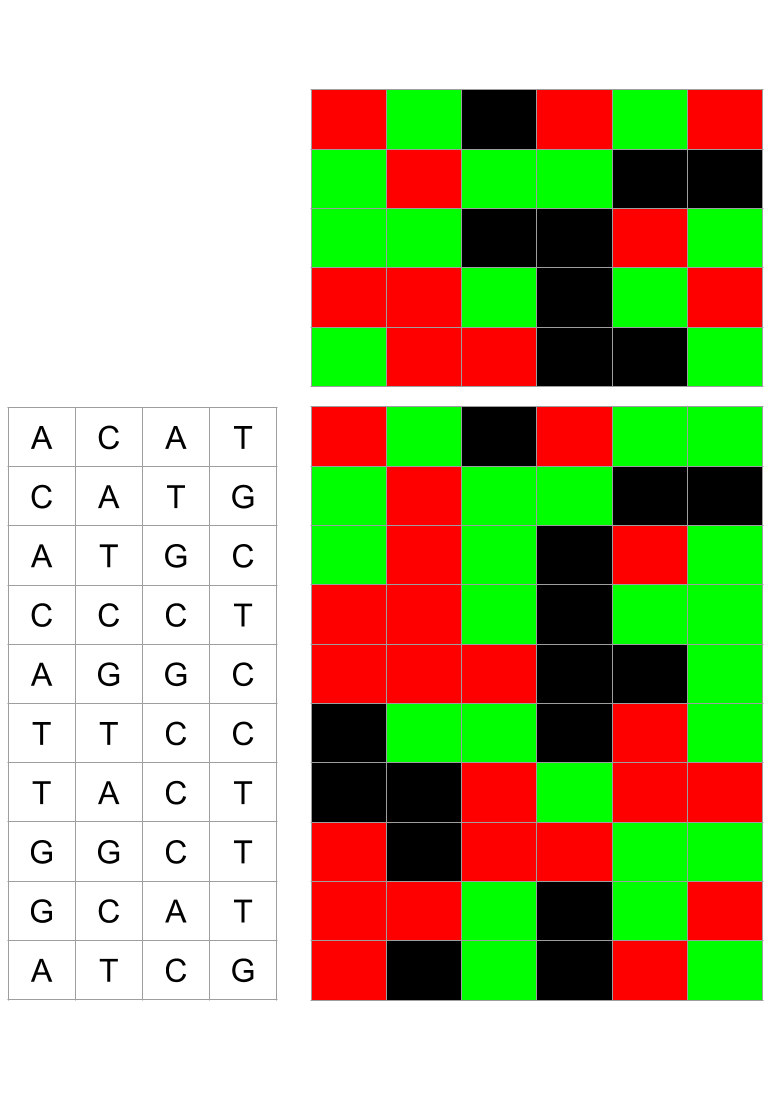
\includegraphics[width=\textwidth]{fig/Dataset.png}
\caption{Dataset}
\label{fig:Dataset}
\end{figure}


\section{Neural Network Architecture}
\label{sec: Neural Network Architecture}
The detailed architecture is in Fig. \ref{fig:Architecture}. All hyperparameters are listed in Table \ref{Hyerparameters}. For simplicity we omitted batch normalization, activation and dropout layers from Table \ref{Hyerparameters}. If not mentioned otherwise, all activations are rectified linear units and all dropout uses a keep rate of 0.5. 


\begin{figure}
\centering
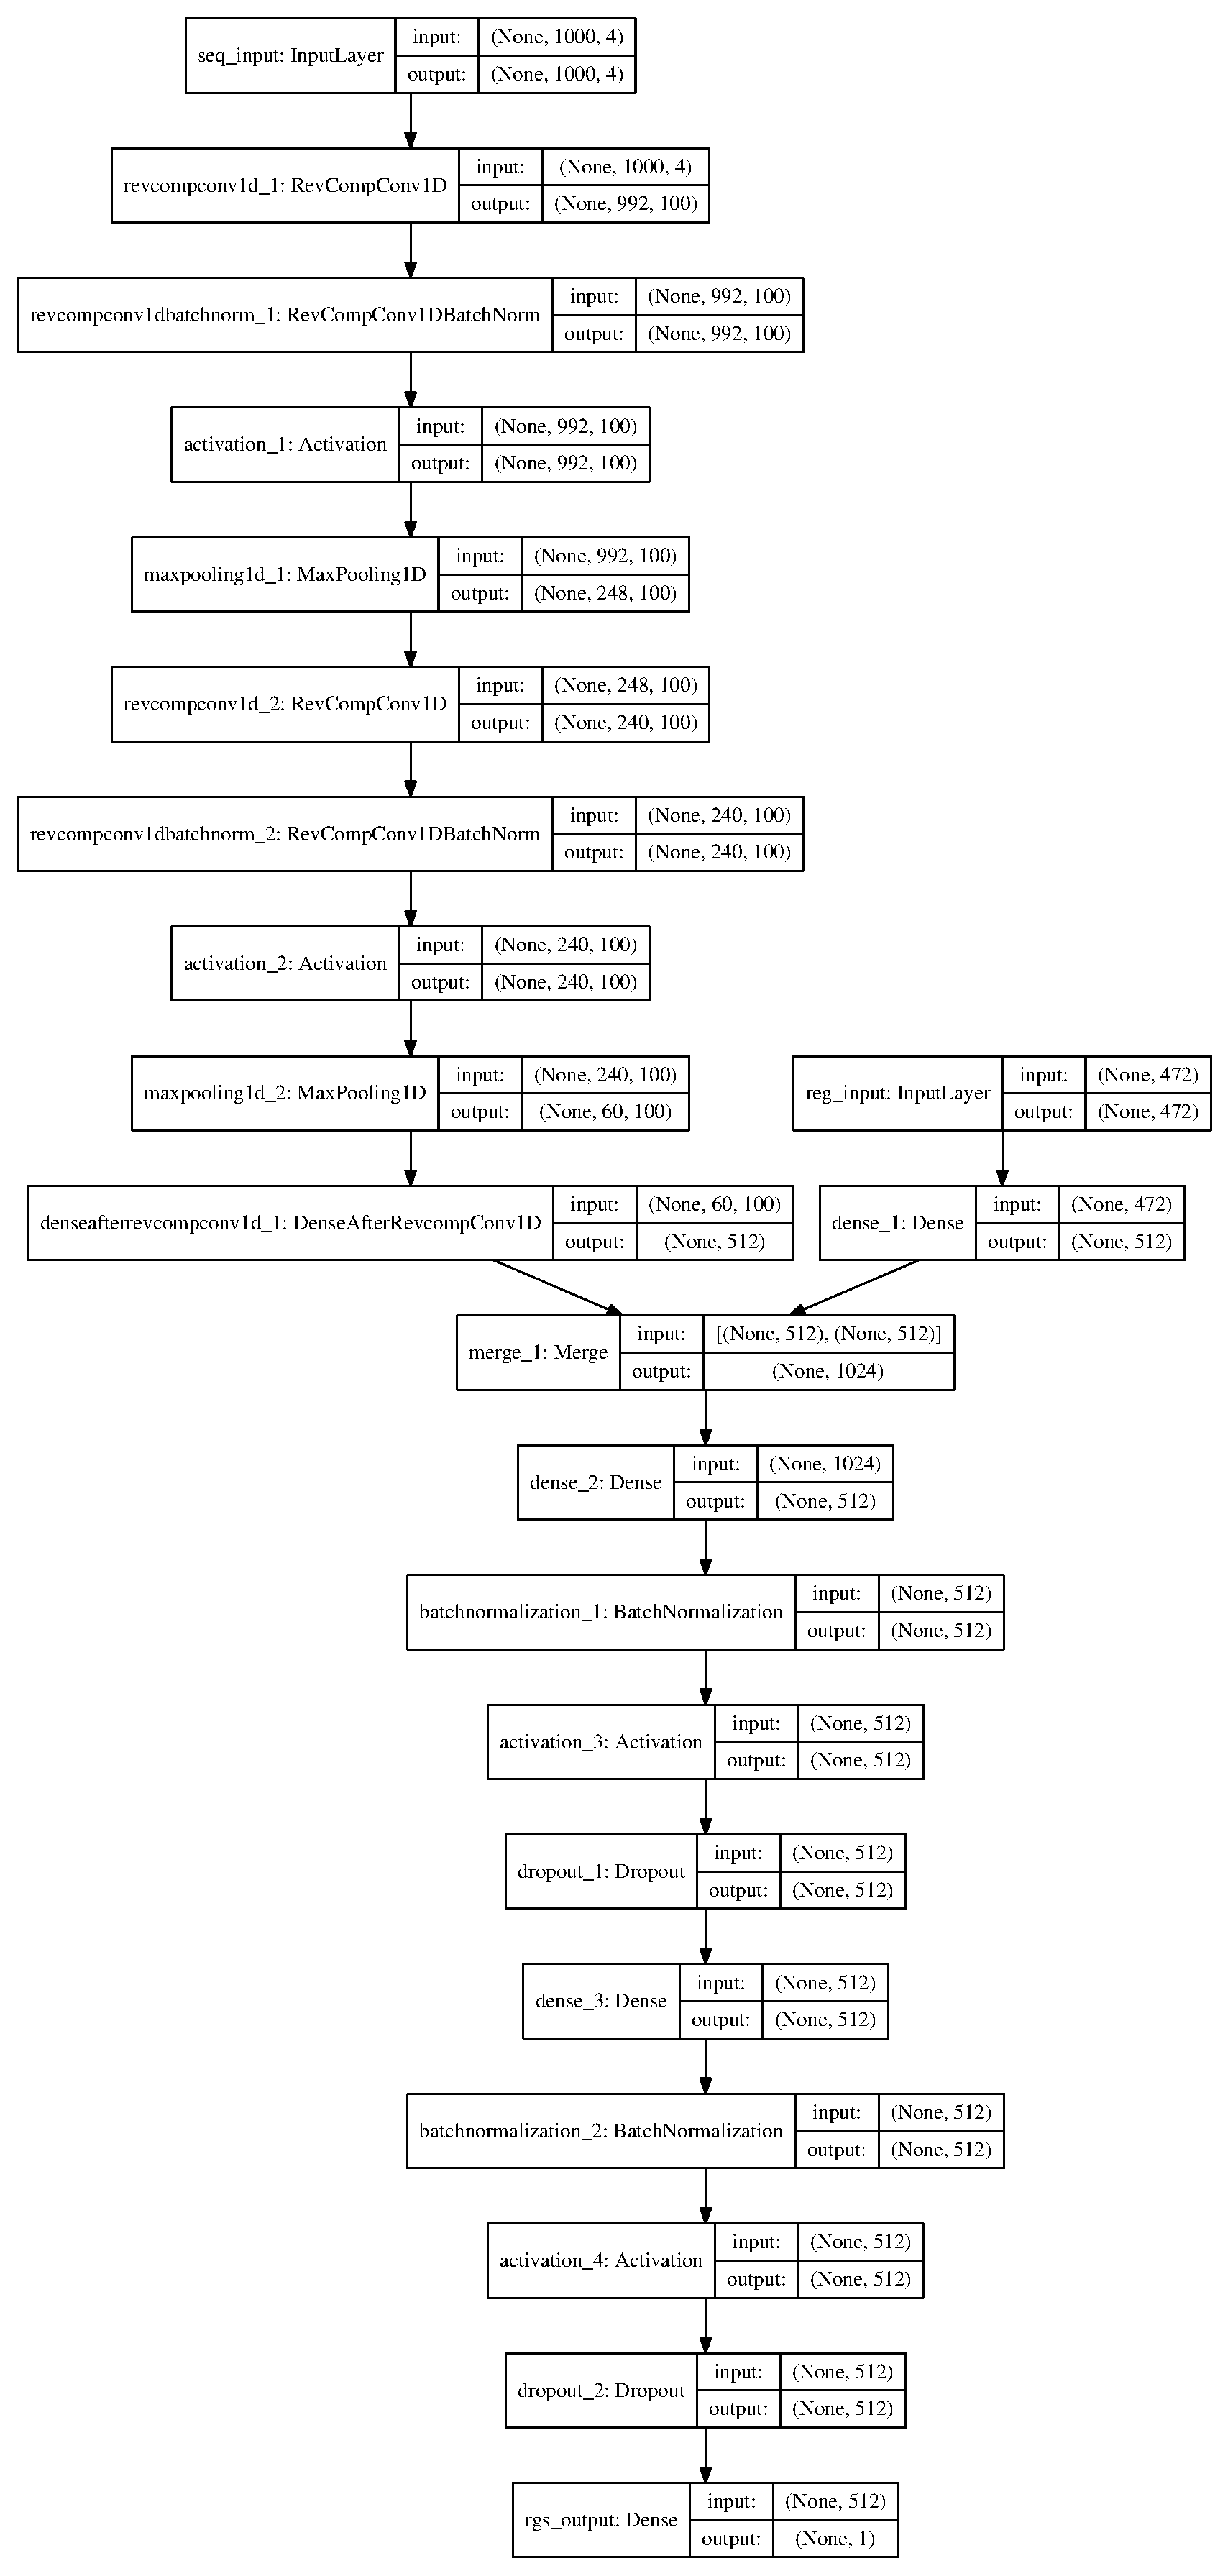
\includegraphics[width=0.8\textwidth]{fig/model.eps}
\caption{Architecture}
\label{fig:Architecture}
\end{figure}


\begin{table}
\centering
\begin{tabular}{| c | c | c | c |}
\hline
Layer & Units & Size & Stride \\
\hline
\hline
\multicolumn{4}{|l|}{Sequence module}\\
\hline
Input & 1000 & - & - \\
\hline
Conv1D & 50 & 9 & 1 \\
\hline
Maxpool1D & - & 4 & 4 \\
\hline
Conv1D & 50 & 9 & 1 \\
\hline
Maxpool1D & - & 4 & 4 \\
\hline
Dense & 512 & - & - \\
\hline
\multicolumn{4}{|l|}{Reg module}\\
\hline
Input & 472 & - & - \\
\hline
Dense & 512 & - & - \\
\hline
\multicolumn{4}{|l|}{Integration module}\\
\hline
Concatenation & 1024 (512 + 512) & - & - \\
\hline
Dense & 512 & - & - \\
\hline 
Dense & 512 & - & - \\
\hline
\end{tabular}
\caption{Hyperparameters}
\label{Hyerparameters}
\end{table}


\section{Motif discovery}
We used a method similar to Basset \cite{Kelley:2016bv} to perform motif discovery. For each convolutional filter, we select the 100 sequence segments with the highest activation. We next calculate the PWM based on nucleotide frequency in these sequence segments. To test whether any PWM correspond to known motif, we used TomTom (http://meme-suite.org/tools/tomtom) to compare against the YEASTRACT database. Below we show several more instances of motif matches. 

\begin{figure}[!tbp]
\centering

\subfloat{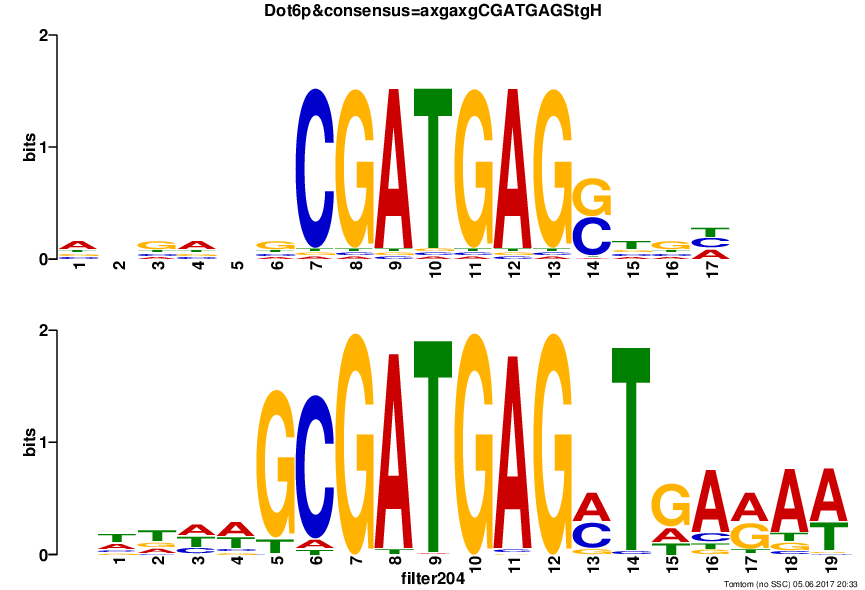
\includegraphics[width=0.2\textwidth]{fig/tomtom/dot6p_2.png}\label{fig:2a}}
\subfloat{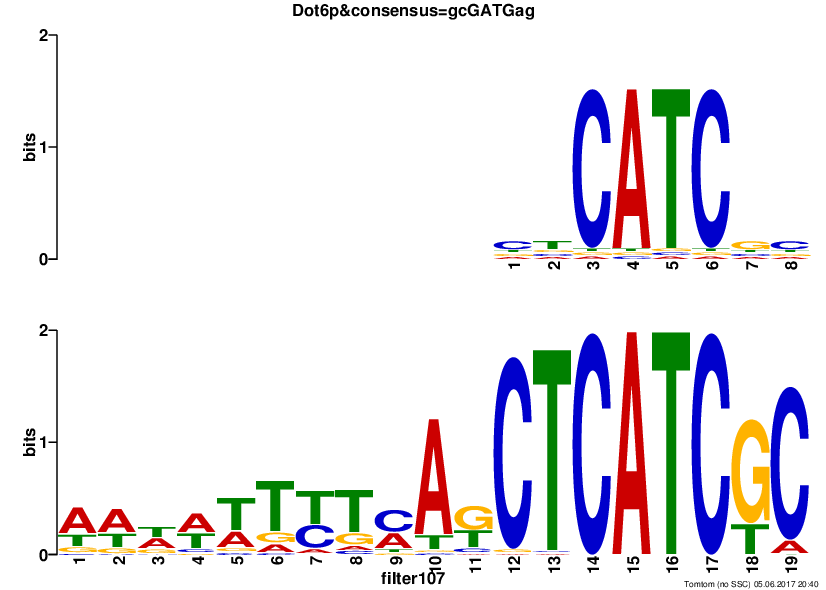
\includegraphics[width=.2\textwidth]{fig/tomtom/dot6p_3.png}\label{fig:2b}}
\subfloat{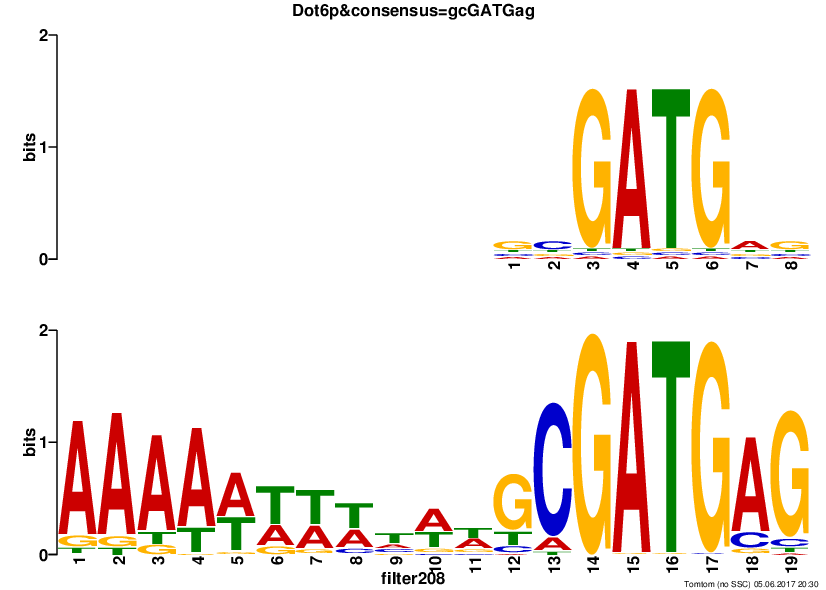
\includegraphics[width=.2\textwidth]{fig/tomtom/dot6p.png}\label{fig:2c}}
\subfloat{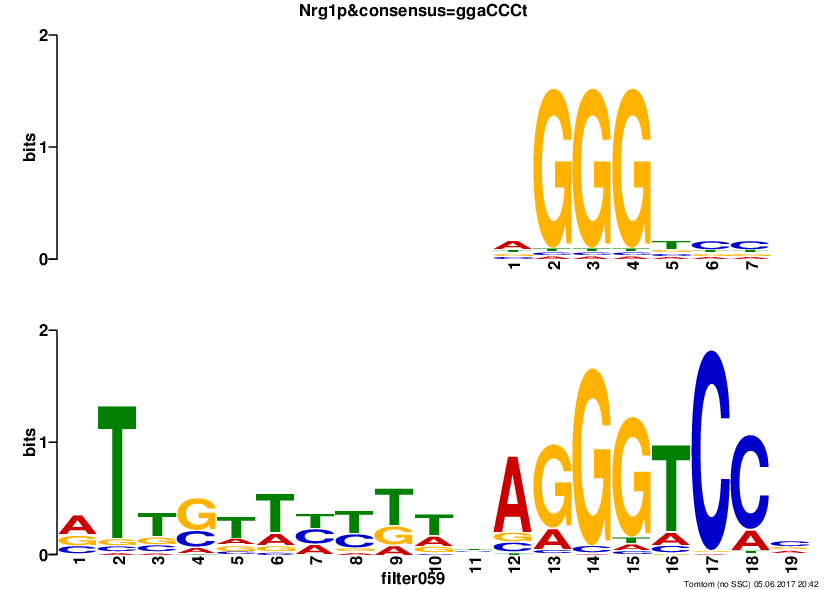
\includegraphics[width=.2\textwidth]{fig/tomtom/nrg1p.png}\label{fig:2d}}


\subfloat{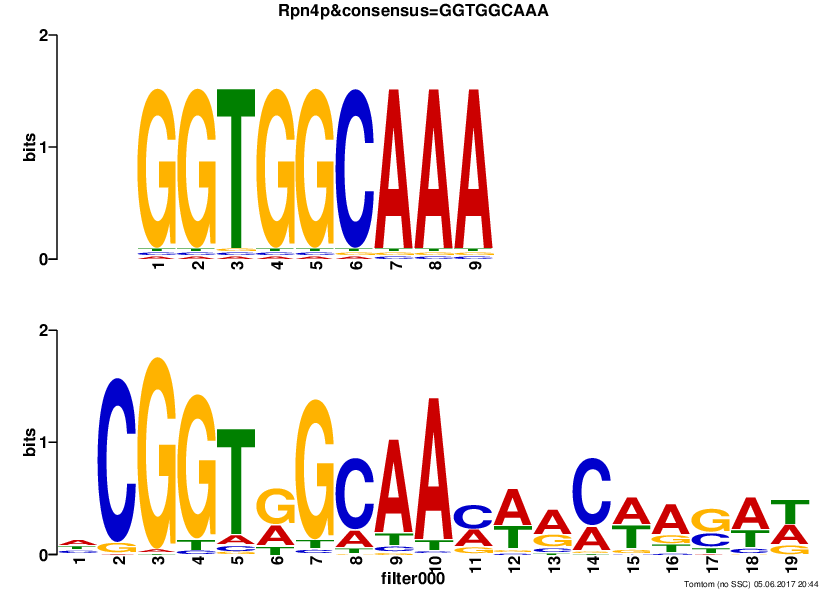
\includegraphics[width=.2\textwidth]{fig/tomtom/rpn4p.png}\label{fig:2e}}
\subfloat{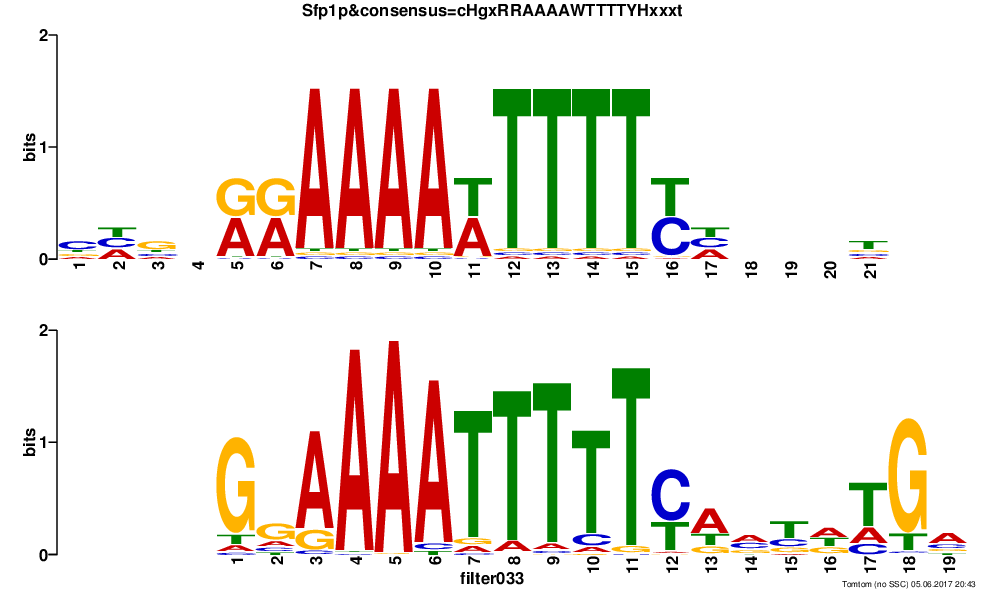
\includegraphics[width=.2\textwidth]{fig/tomtom/sfp1p_2.png}\label{fig:2f}}
\subfloat{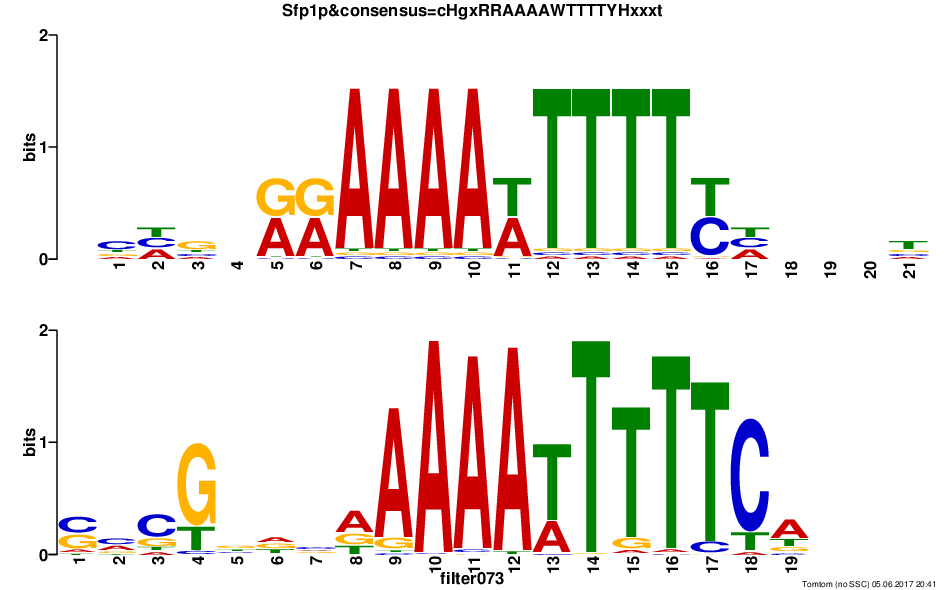
\includegraphics[width=.2\textwidth]{fig/tomtom/sfp1p.png}\label{fig:2g}}
\subfloat{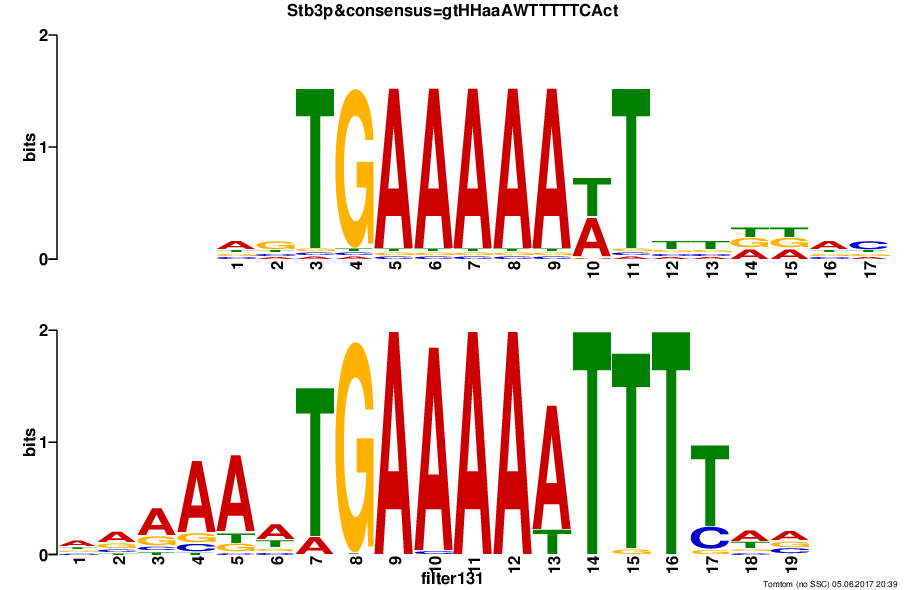
\includegraphics[width=.2\textwidth]{fig/tomtom/stb3p.png}\label{fig:2h}}

\caption{Example of known motifs recovered by the convolutional filters}
\end{figure}


\section{Ranking regulator by feature importance}
To understand which transcription factors and/or signaling molecules are most predictive, we used a backpropagation approach to rank the each input to the regulatory module \cite{Shrikumar:2016uy}. We reasoned that perturbation to highly influential features would lead to large change in the output. We quantified the feature importance using gradient (w.r.t output) times the input \cite{Samek:2016hk}. To get the overall importance, we summed the gradient times input across all conditions and all genes. 


\section{\textit{in silico} Mutagenesis}
To test whether our model makes biologically relevant predictions, we decided to compare \textit{in silico} MSN2/4 knockout against actual microarray measurement. MSN2/4 are two master transcription regulators with about 300 target genes. They are only activated under stress conditions such as heat shock. We removed the MSN2/4 binding sequence ('AGGGG' and its reverse complement sequence) and reduced the expression by 32 fold. Since MSN2/4 are only activated under stress conditions, we expect that the expression of their target genes will have larger change under stress than normal growth conditions. As expected, in heat shock experiments (the first five groups), MSN2/4 target genes show more pronounced decreases in expression values compared with non-target genes. This indicates that MSN2/4 has a greater influence in known target genes (Fig. \ref{msn24_ko_target_genes_2msn24_ko_target_genes_2}). As a negative control, we looked at steady-state growth conditions. In these conditions, since MSN2/4 are not activated, knocking them down should not influence the target genes. Indeed, we observe smaller differences in the next five groups, which are steady-state growth experiments. In addition, the smaller errorbars indicate smaller overall effect by MSN2/4 knockdown. The same pattern can be observed for the last five groups corresponding to exponential growth conditions at different temperature. Notably, the last group, exponential growth at 37 C, shows a pattern close to a heat shock experiment. We reason that heat-shock experiments are generally conducted by raising culturing temperature temporarily to 37 C, and exponential growth at this temperature disrupts the normal function of the yeast regulatory machinery, thus activating MSN2/4. Fig. \ref{msn24_ko_target_genes} shows the difference in mean between MSN2/4 target and non-target genes. The heat shock experiments clearly show greater differences than steady-state and exponential growth conditions. Interestingly, as the heat shock becomes milder, the difference becomes smaller. Again, we observe that 37 C growth is similar to heat shock. 

\begin{figure}


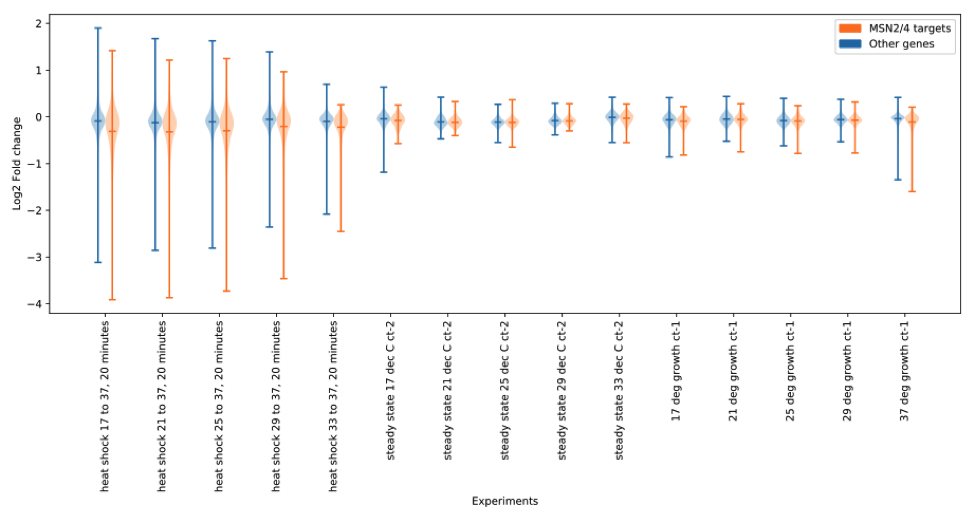
\includegraphics[width=\textwidth]{fig/msn24_ko_target_genes_2.png}
\caption{Distribution of change in expression stratified by MSN2/4 target or non-target genes}
\label{msn24_ko_target_genes_2}


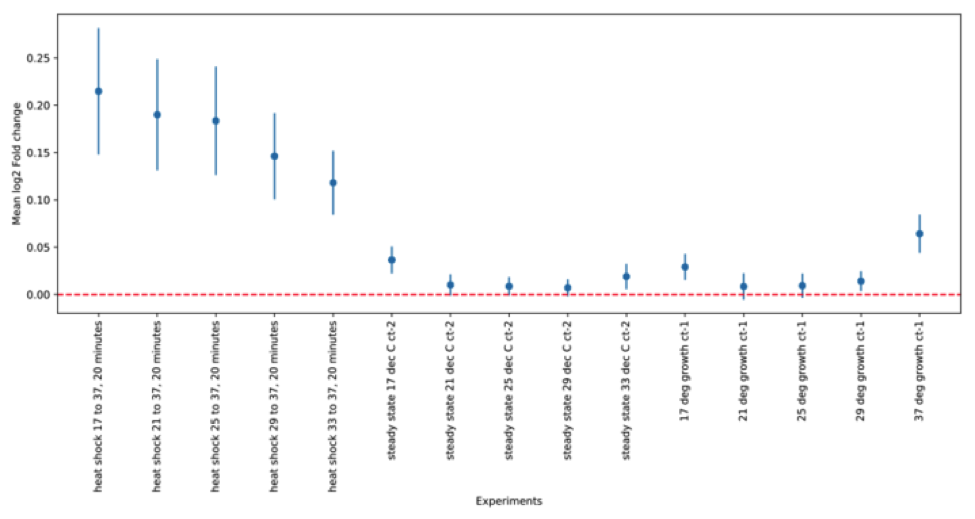
\includegraphics[width=\textwidth]{fig/msn24_ko_target_genes.png}
\caption{Difference of change in expression between by MSN2/4 target and non-target genes}
\label{msn24_ko_target_genes}

\end{figure}

As an orthogonal validation, we performed \textit{in silico} MSN2/4 knockout experiments for yeast exposed to 37C heat shock. The resultant predictions were compared with actual MSN2/4 strains exposed to 37 C heat shock. We ranked the genes according to the changes in their expression - downregulation is ranked higher than upregulation. Their rank correlation is shown below as a smoothed scatter plot. The rank is consistent for extreme upregulated/downregulated genes. However, for genes whose expression underwent less dramatic change, the prediction can be noisy. We reason that this is due to regulatory buffering. Genes with large expression change are often directly regulated by MSN2/4, where those with smaller change are indirectly regulated through intermediate genes. Since we only knock out MSN2/4, directly regulated genes will be strongly affected, and therefore show consistency with microarray measurement. On the other hand, the effect of MSN2/4 knockout may not penetrate deep enough to indirectly regulated genes due to regulatory buffering. 

\begin{figure}
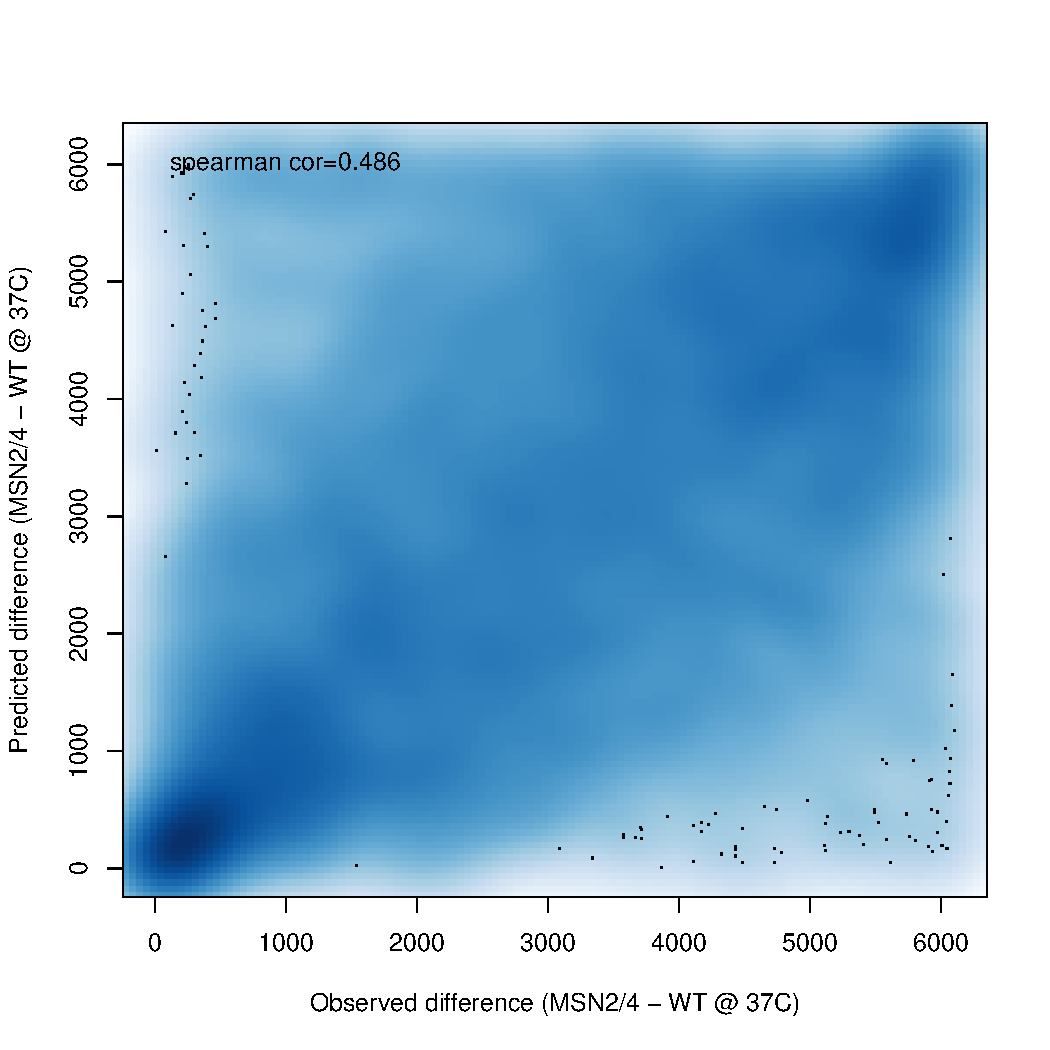
\includegraphics[width=\textwidth]{fig/msn24_ko_37C_diff_expr_rank.pdf}
\caption{Comparison of \textit{in silico} knockout and microarray measurement}
\label{msn24_ko_37C_diff_expr_rank}
\end{figure}



\bibliographystyle{unsrt}
\bibliography{references}

\end{document}